\documentclass[a4paper]{jpconf}
\usepackage{graphicx}
\bibliographystyle{iopart-num}



\begin{document}
\title{Development of Machine Learning Tools in ROOT}

\author{S. V. Gleyzer$^1$, L. Moneta$^2$, Omar A. Zapata$^3$, }




\address{$^1$ University of Florida}

\address{$^2$ CERN}

\address{$^3$ University of Antioquia and Metropolitan Institute of Technology}


\ead{Sergei.Gleyzer@cern.ch, Lorenzo.Moneta@cern.ch, Omar.Zapata@cern.ch}




\begin{abstract}
ROOT is a framework for large-scale data analysis that provides basic and advanced statistical methods used by the LHC experiments. In particular, these include machine learning algorithms from the ROOT-integrated Toolkit for Multivariate Analysis (TMVA). We present recent developments in TMVA as well as the interfaces between ROOT and other statistical tools, such as R.
\end{abstract}



\section{Introduction}
ROOT is a modular object-oriented C++ data analysis framework that provides statistical methods, advanced visualization and storage libraries for the data analysis of High-Energy Physics (HEP) experiments \cite{Antcheva20092499}. TMVA is a ROOT-integrated toolkit that implements Machine-learning algorithms \cite{Hocker:2007ht}. Figure \ref{tmva:label} shows the interfaces between ROOT, TMVA and other statistical tools. As part of the Machine-learning Toolbox, TMVA provides a set of algorithms widely used in High Energy Physics (HEP):

\begin{itemize}  
\item Boosted Decision Trees (BDT)
\item Artificial Neural Networks (ANN)
\item Support Vector Machines (SVM)
\item and others
\end{itemize}
Recently TMVA has  been undergoing a lot of improvements targeting  greater flexibility, more modular design and novel features and interfaces. In the next sections we describe some of the new features and functionality of TMVA.


\begin{figure}[h]
\centering
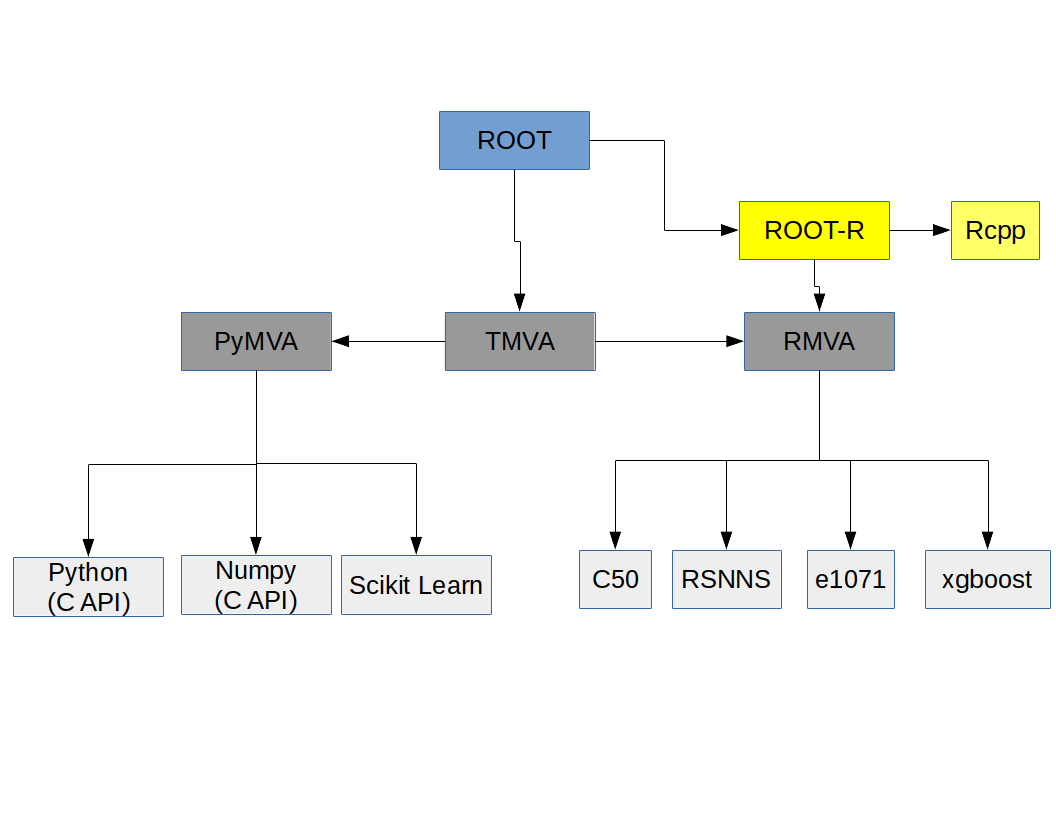
\includegraphics[width=25pc]{img/tmva.png}\caption{\label{tmva:label} Machine Learning Tools in ROOT.}
\end{figure}

\subsection{DataLoader}
DataLoader is a new class in TMVA that allows greater modularity and flexibility for training different classifiers with different features. With DataLoaders a user defines which data and features will be used during training. Multiple DataLoaders are allowed at the same time. Figures \ref{dl1}, \ref{dl2} and \ref{dl3} show the structure of the TMVA::Factory class and the new DataLoader class. The DataLoader class currently supports ROOT and comma-separated value (csv) files.


\begin{figure}[h]
\begin{minipage}{15pc}
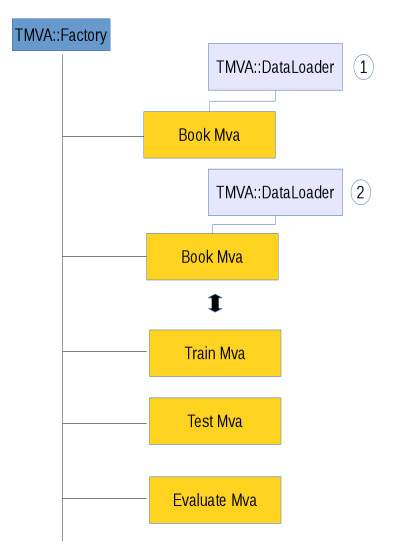
\includegraphics[width=15pc]{img/dl1.jpg}
\caption{\label{dl1}Booking methods with different dataloaders}
\end{minipage}\hspace{2pc}%
\begin{minipage}{15pc}
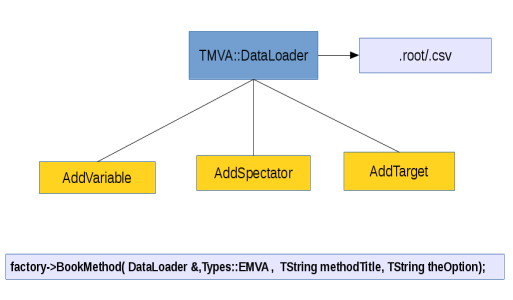
\includegraphics[width=20pc]{img/dl2.jpg}
\caption{\label{dl2}Loading data from files.}
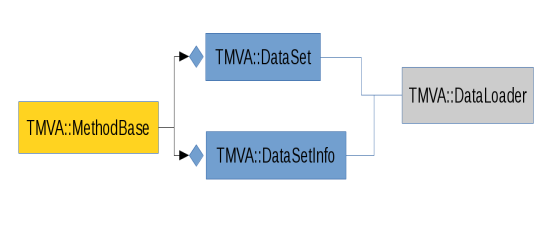
\includegraphics[width=20pc]{img/dl3.jpg}
\caption{\label{dl3}Storing data in objects in the class MethodBase.}
\end{minipage} 
\end{figure}


\subsection{Variable Importance}
In addition to increasing TMVA modularity, a number of algorithms providing user with useful information have been added. For example, a stochastic algorithm described in \cite{gleyzer2008paradigm} for computing variable importance, 
has been implemented in TMVA. Figure \ref{vi} shows a sample variable importance plot for a basic example in TMVA.

\clearpage
\begin{figure}[h]
\centering
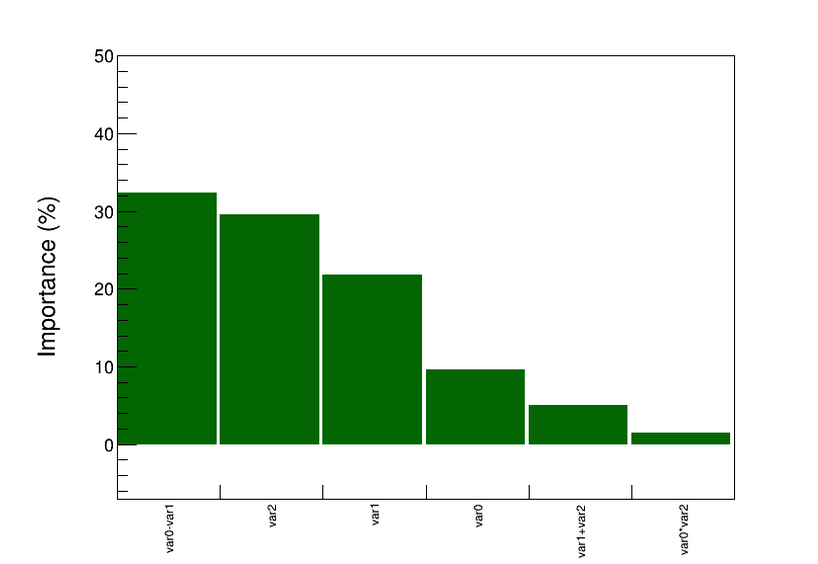
\includegraphics[width=25pc]{img/vi.png}\caption{\label{vi} Histogram ranking the variables.}
\end{figure}


\subsection{ROOT-R and RMVA}\label{ROOTR}
R  is a free software framework for statistical computing\cite{R}. We developed the ROOT-R package which allows the  use of R functions directly in ROOT. This interface opens a large set of statistical tools in R for use within ROOT. The ROOT-R interface design is shown in Figure \ref{rootr:label}. 


\begin{figure}[h]
\centering
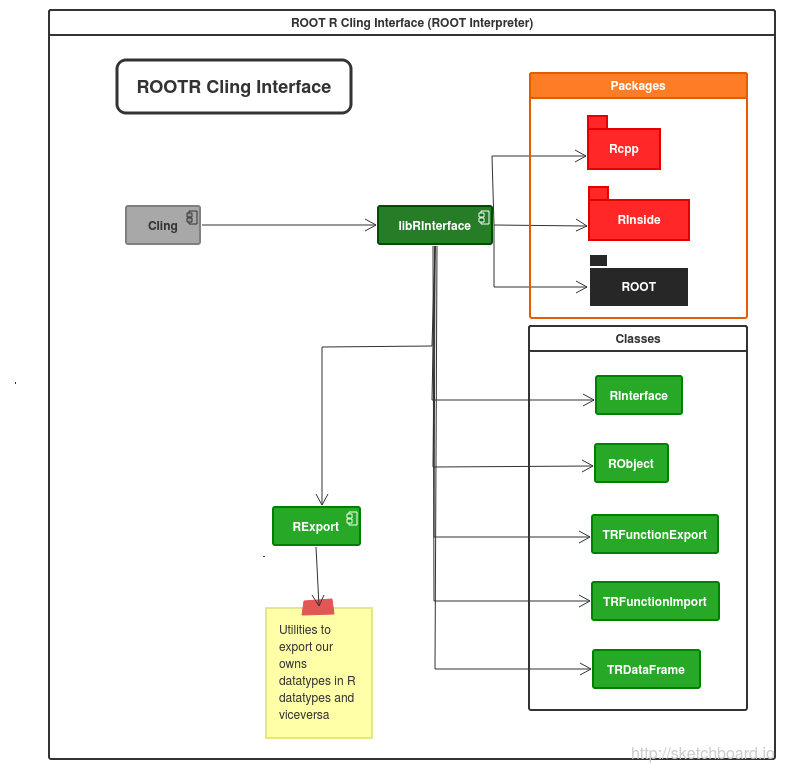
\includegraphics[width=25pc]{img/rootr.png}\caption{\label{rootr:label} ROOT-R design.}
\end{figure}
RMVA is a set of plugins for TMVA based on the ROOT-R interface. RMVA allows the use of machine-learning methods in R in TMVA.  Each of the methods inherits from the base class RMethodBase as shown in Figure \ref{rmvaplug}. Currently, the following methods are supported: 

\begin{itemize}  
\item C5.0 decision trees and rule-based models (C500 \cite{c50}.
\item Stuttgart Neural Networks in R (SNNS)\cite{rsnns}.
\item Support Vector Machines in R (e1071)\cite{e1071}.
\item eXtreme Gradient Boost (xgboost) An optimized
general purpose gradient boosting library\cite{chen2015xgboost}.
\end{itemize}
Various machine-learning methods from R can be tried within the TMVA framework, as shown in Figure \ref{rmvaroc}.



\begin{figure}[h]
\centering
\begin{minipage}{15pc}
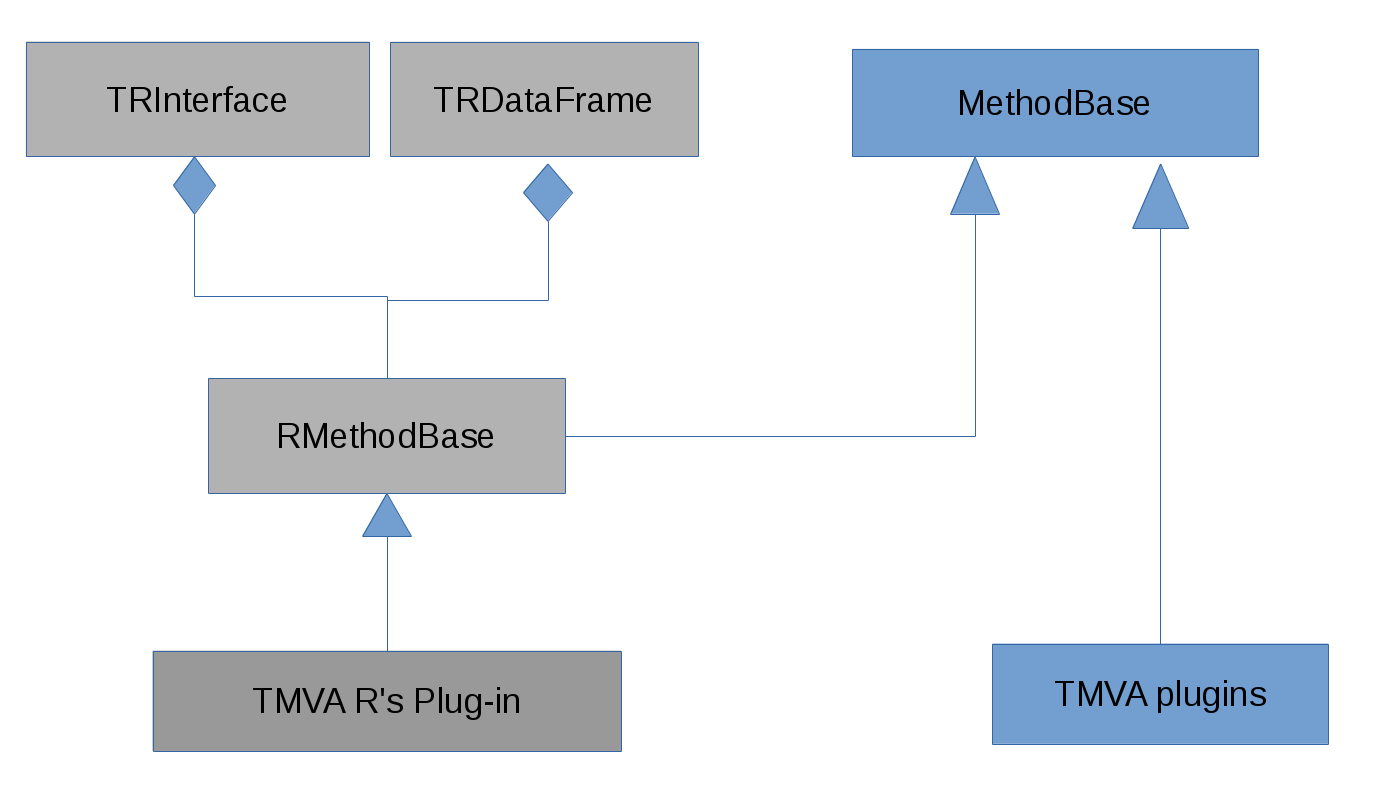
\includegraphics[width=16pc]{img/rmvaplugins.png}
\caption{\label{rmvaplug}ROOTR and TMVA plugins system}
\end{minipage}\hspace{2pc}%
\begin{minipage}{15pc}
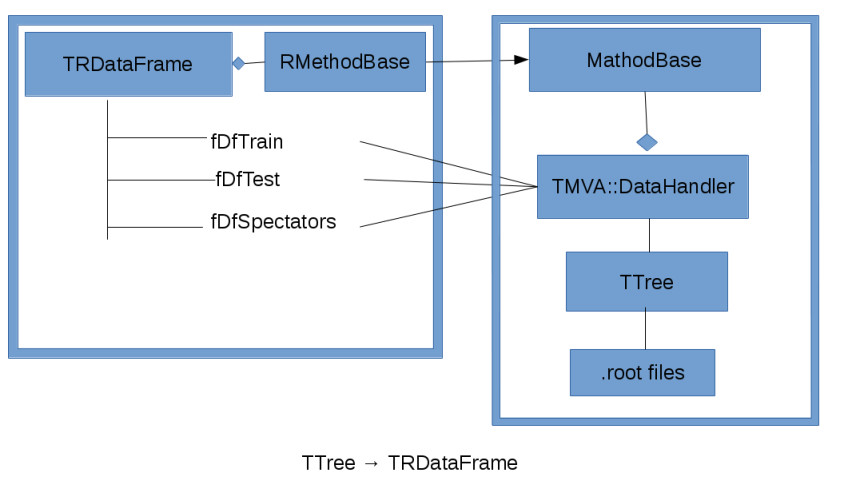
\includegraphics[width=16pc]{img/rmvadf.jpg}
\caption{\label{rmvadf}ROOTR and TMVA data flow.}
\end{minipage}\hspace{2pc}%
\end{figure}



\begin{figure}[h]
\centering
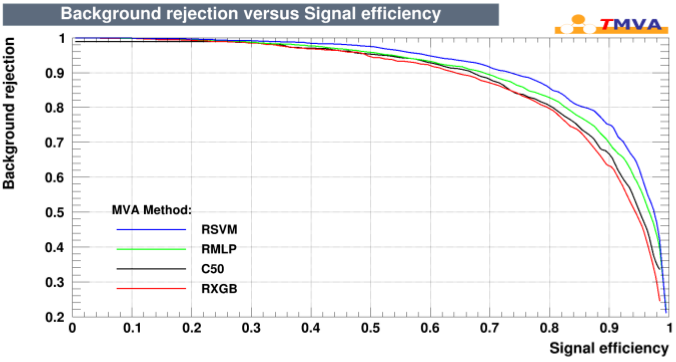
\includegraphics[width=25pc]{img/rmvaroc.png}\caption{\label{rmvaroc} ROC Curves for RMVA methods}
\end{figure}

\subsection{Python with TMVA (PyMVA)} \label{PYMVA}
PyMVA is a set of TMVA plugins based on Python API that opens additional machine-learning methods written in Python to be used from TMVA. Each PyMVA method inherits from the base class PyMethodBase, as illustrated in Figure \ref{pymvaplug}. Figure ref{pymvadf} shows how PyArrayObject class is used to map the dataset from ROOT trees to numpy arrays. The following python-based methods from \cite{pedregosa2011scikit} are currently available in TMVA:


\begin{itemize}
\item Random Forest (PyRandomForest)
\item Gradient Boosted Regression Trees (PyGTB) 
\item Adaptive Boosting (PyAdaBoost) 
\end{itemize}
Figure \ref{pymvaroc} shows the ROC curves of various PyMVA methods for a basic example.



\begin{figure}[h]
\centering
\begin{minipage}{15pc}
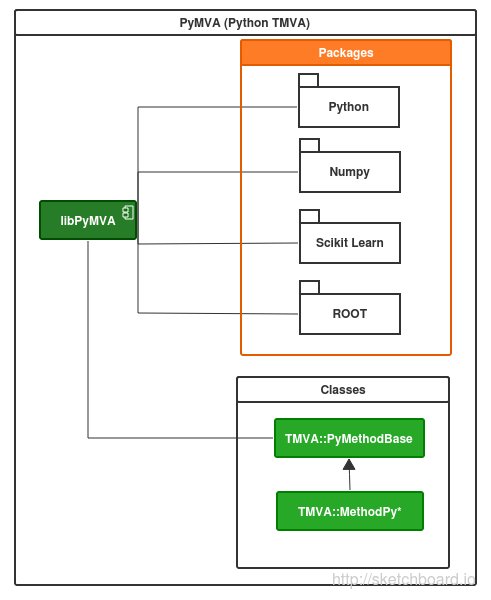
\includegraphics[width=16pc]{img/pymvaplugins.png}
\caption{\label{pymvaplug}Python and TMVA plugins system}
\end{minipage}\hspace{2pc}%
\begin{minipage}{15pc}
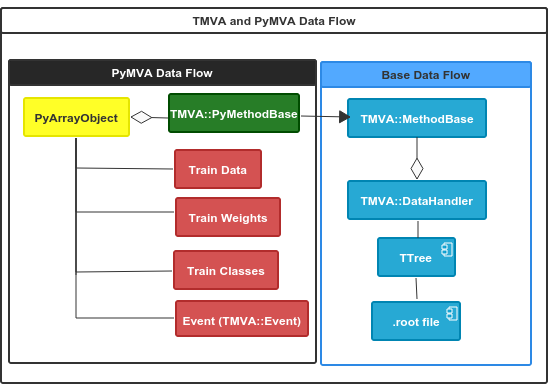
\includegraphics[width=16pc]{img/pymvadf.png}
\caption{\label{pymvadf}Python and TMVA data flow.}
\end{minipage}\hspace{2pc}%
\end{figure}


\begin{figure}[h]
\centering
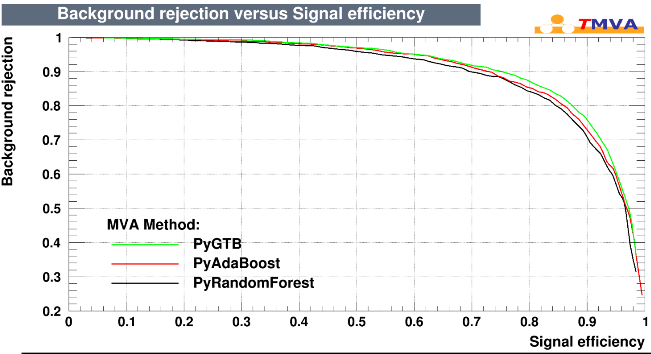
\includegraphics[width=25pc]{img/pymvaroc.png}\caption{\label{pymvaroc} ROC Curve for TMVA methods with Python.}
\end{figure}

\clearpage
\subsection{Acknowledgments}
The work of Omar. A. Zapata has been partially supported by Sostenibilidad-UdeA, UdeA/CODI grant IN361CE
and COLCIENCIAS through the grant number 111-556-934918.\newline
Computer Science Center, Metropolitan Institute of Technology - Medellin/Colombia.


\section*{References}
\bibliography{iopart-num}

\end{document}

% \end{document}











